 \documentclass[12pt ]{article}
 \usepackage[table]{xcolor}
\usepackage[slovene]{babel}
\usepackage{color}
\usepackage{graphicx}
\usepackage{subfigure}
\usepackage{gensymb}
\usepackage{amssymb} % za simbol za realna števila
\usepackage{indentfirst}
\usepackage{fullpage} 
\usepackage{hyperref}
\usepackage{musicography}
\usepackage[utf8]{inputenc}
\usepackage{amsmath} % za boldmath{}
\usepackage{float} % ce das [H] pri sliki ali tabeli jo postavi tocno tam v besedilu
\usepackage{siunitx} % za pravi typesetting enot
\usepackage{physics} % za previ typesetting diferencialov
\usepackage{xcolor} % da oznacim, kaj sem na novo jaz napisal, da lahko kdo pregleda brez precesavanja celega teksta
\usepackage{subcaption} % za slikce na isti visini
% blue - pisal Jon
% purple - pisal Fedja
% orange - samo komentar
\usepackage{footnote}
%\usepackage[font={small,it}]{caption} %da se ve kaj je caption
\makesavenoteenv{tabular}
\makesavenoteenv{table}
\usepackage[style=numeric,backend=biber,sorting=none]{biblatex} % za citiranje. IZI citiranje: https://tex.stackexchange.com/questions/3833/how-to-cite-an-article-from-arxiv-using-bibtex
\addbibresource{Viri.bib}
\usepackage{amssymb}
\usepackage{amsmath}
\usepackage{geometry}
\geometry{
 a4paper,
 total={160mm,240mm}  
  }
 
 \begin{document}
 $~$ 
 
 \vspace{2cm}
 
 \centerline{\bf \huge  Optične metaleče}
 
 \vspace{1cm}
 
  \centerline{\huge  Matic Tonin}
  
   \vspace{1cm}
  
  \centerline{\large Mentor: Daniel Svenšek}
  
  \vspace{1cm}
  
  \centerline{\large Seminar, 3. letnik}
  
  \vspace{1cm}
  
  \centerline{\large Oddelek za fiziko, FMF, UL, 2021/2022}
  
  \vspace{6cm}
  
  \begin{minipage}[c]{0.9\hsize}
  {\bf Povzetek}
  Optične metaleče so ultratanke optične površine, ki so sposobne upravljanja različnih lastnosti svetlobe, kot so faza, polarizacija, amplituda ... S tem predstavljajo alternativo klasičnim lečam in ostalim optičnim elementom, ki jih imamo v optičnih napravah. Njihove lastnosti izvirajo iz zgradbe in postavitve njihovih notranjih elementov. Metaleče so zgrajene iz umetnih materialov, kot sta TiO$_2$ in Ga-N, ki s pravilno postavitvijo v hiperboličen ali kvadratičen profil zagotavljata konstruktivno interferenco v goriščni razdalji leče. Zaradi odvisnosti faznega zamika od valovne dolžine svetlobe se znanstveniki soočajo s problemom realizacije metaleč za široke spektre in iščejo alternative, kako bi izboljšali izkoristek delovanja metaoptičnih površin.
    \end{minipage}

 
 \newpage
  
  
 \section{Uvod}
 Optični elementi igrajo ključno vlogo v današnjem svetu, saj jih srečamo skoraj povsod, od pametnih telefonov pa vse do raketnih izstrelkov. Zaradi napredka v tehnologiji in miniaturnosti naprav, ki jih uporabljamo, se optika sooča z velikim problemom, saj so klasične leče in ogledala precej okorna in velika. Za primer razvoja optične tehnologije si lahko pogledamo sliko \ref{Opticna_zgodovina}. Za začetek so bile v uporabi navadne steklene leče, pri katerih velja, da bolj ukrivljena površina povzroči močnejši lom svetlobe. S tem pa se pojavi problem, da je za močnejše lome potrebna velika debelina leče in zato so začeli uporabljati periodične uklonske mrežice ali uklonske leče (kar prikazuje slika \ref{Opticna_zgodovina} (c)), ki so rešile problem večanja debeline inštrumenta. Te morajo s pravimi faznimi zamiki zagotoviti, da tisti žarki, ki gredo skozi gorišče, v gorišču pozitivno interferirajo. Žarek ob prehodu skozi lečo prejme fazni zamik
 \begin{equation}
 \Delta=\frac{2\pi(n-1)t}{\lambda},
 \end{equation} 
kjer $t$ predstavlja debelino leče (slika \ref{Opticna_zgodovina}(c)), $n$ je lomni količnik in $\lambda$ valovna dolžina vpadne svetlobe. Fazni zamik, ki ga mora takšna leča ustvariti, mora segati vse od 0 pa do $2\pi$. S tem mora biti debelina leče vsaj
 \begin{equation}
     t=\frac{\lambda}{(n-1)}.
 \end{equation}
Tako je svetloba pri prehodu skozi uklonsko lečo pridobila fazni skok. Kasneje se je začelo uporabljati večslojne uklonske mrežice \textit{Multilevel diffractive lenses ali MDLs} \ref{Opticna_zgodovina}(d). Njihova stopničasta zgradba ustvarja skoraj zvezen fazni skok, ki omogoča boljši izkoristek leče, njihov glavni problem pa je zbiranje svetlobe pod velikimi vpadnimi koti.
 \begin{figure}[H]
     \centering
     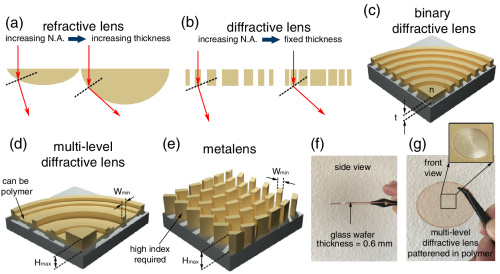
\includegraphics[width=12cm, height=7cm]{Slike/Opticna zgodovina.jpg}
     \caption{Prikaz različnih metod loma svetlobe, a) na stekleni leči, b) na uklonski mrežici, c) na uklonski leči, d) na večslojni uklonski leči in e) na metaleči. Sliki f) in g) prikazujeta velikosti večslojne uklonske leče. Vir: \cite{Zgodovina} }
     \label{Opticna_zgodovina}
 \end{figure}
Raziskovanje tanjšanja optičnih naprav in širjenja spektra valovnih dolžin, ki ga lahko opazujemo z inštrumentom, se je nato nadaljevalo in privedlo do razvoja metaleč \cite{Zgodovina}.
 
 \section{Metaleče, njihovo delovanje in zgradba}
 Metaleče spadajo v skupino metapovršin. Metapovršine so umetno zgrajeni materiali, sestavljeni iz 2D periodičnih kovinskih ali dielektričnih nanostruktur.
 
 
 
 

\subsection{Osnove optičnih površin}
Za lažje razumevanje delovanja metaleč si bomo najprej pogledali, kako se svetloba ukloni na krožni uklonski mrežici. 


Za svetlobo, ki seva iz točkastega izvora vemo, da njena amplituda $\psi$ ustreza rešitvam Helmholtzeve enačbe:
\begin{equation}
\nabla^{2} \psi+k^{2} \psi=\delta(\mathbf{r}) \quad \psi(r)=\frac{e^{ikr}}{4\pi r},
\end{equation}
kjer je $k$ valovni vektor in $r$ razdalja od izvora.
\begin{figure}[H]
    \centering
    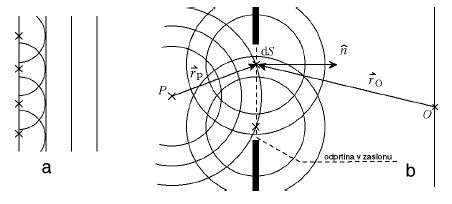
\includegraphics{Slike/pRAK.JPG}
    \caption{(a) V ravnem valu si lahko predstavljamo vsak del valovne fronte kot izvor krogelnega vala. Vsota teh krogelnih valov je ponovno ravna valovna fronta. (b) Točkast izvor P oddaja krogelni val. Vse točke znotraj odprtine v zaslonu so izvori novih krogelnih valov. Uklonsko sliko dobimo s seštevanjem amplitud teh krogelnih valov. Vir: \cite{Praktikum4}.}
    \label{Slika uklona}
\end{figure}

Po Huygensovim načelu lahko vsako točko na valovni fronti obravnavamo kot točkast izvor z amplitudo $\psi$ (glej sliko\ref{Slika uklona}(a)). Ko valovna fronta naleti na zaslon z odprtino, se valovanje na zaslonu delno odbije in absorbira, v območju odprtine pa imamo sekundarne izvore valovanja, kar ilustrira slika \ref{Slika uklona}(b). V primeru pravokotnega vpada svetlobe z amplitudo električnega polja $E_{\text {inc }}$ na uklonsko režo je amplituda novega valovanja enaka
\begin{equation}
\Psi(r) \propto \iint_{\text {Reža }} E_{\text {inc }}\left(x^{\prime}, y^{\prime}\right) \frac{e^{i k\left|\mathbf{r}-\mathbf{r}^{\prime}\right|}}{4 \pi\left|\mathbf{r}-\mathbf{r}^{\prime}\right|} d x^{\prime} d y^{\prime}
\label{Reza}
\end{equation}
kjer je $\mathbf{r}$ vektor od izvora do vpada na mrežico in $\mathbf{r}^{\prime}$ vektor od središča reže do točke vpada \cite{Praktikum4}. V primeru velike oddaljenosti od reže se tako člen razdalje poenostavi v $\left|\mathbf{r}-\mathbf{r}^{\prime}\right| \approx \mathbf{r}$, če pa še upoštevamo, da je uklonska reža dvodimenzionalna, se enačba \eqref{Reza} preoblikuje v
\begin{equation*}
\Psi(r) \propto \frac{e^{i k r}}{4 \pi r} \iint_{\text {Reža }} E_{\text {inc }}\left(x^{\prime}, y^{\prime}\right) e^{-i\left(k_{x} x^{\prime}+k_{y} y^{\prime}\right)} d x^{\prime} d y^{\prime}, \quad 
k_{x}=k \sin \theta \cos \phi,
k_{y}=k \sin \theta \sin \phi.
\end{equation*}

\begin{figure}[H]
    \centering
    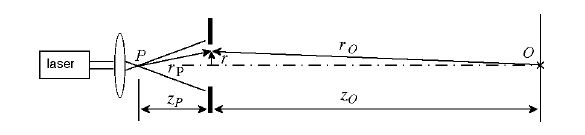
\includegraphics{Slike/Uklonska.JPG}
    \caption{Uklon na okrogli odprtini. Fokusiran laserski snop se iz gorišča leče širi kot krogelni val. Izvor P in točka opazovanja O ležita na osi okrogle odprtine. Vir: \cite{Praktikum4}}
    \label{Uklon}
\end{figure}
Če uporabljamo krožne odprtine z radijem $r$, kot prikazuje slika \ref{Uklon}, lahko opazimo, da bo zaradi simetrije problema veljalo $k_x=k_y=k$. Tako bo amplituda nastalega valovanja $\Psi$ enaka
\begin{equation}
    \Psi\propto \frac{e^{i k r_p}}{4 \pi r_p}\iint_{\text {Reža }} E_{\text {inc }} \frac{E^{ikr_o}}{r_o}\text{d}S
    \label{Krogelna}
\end{equation}
in razvidno je, da je odvisna zgolj od tega, kolikšen je $r$ (radij krožne odprtine), ki se skriva v $\text{d}S$. Okroglo odprtino lahko tako razdelimo na kolobarje (Fresnelove cone), ki sevajo valovanje z približno enako fazo. Da bi izračunali, kolikšna je fazna razlika med središčnim vpadnim žarkom in žarkom, ki se je uklonil na kolobarju, si lahko pogledamo sliko \ref{Uklon}. Razberemo lahko, da razlika optičnih poti znaša
\begin{equation}
    (r_p+r_o)-(z_o+z_p)=m\frac{\lambda}{2}.
\end{equation}
Z upoštevanjem, da so razdalje med objekti ($r_o,r_p$) veliko večje kot reža $r$ \footnote{S to predpostavko je Taylorjev razvoj pitagorovega izreka enak $r_o=\sqrt{z_o^2+r^2}\approx z_o+r^2/2z_o$ in $r_p=\sqrt{z_p^2+r^2}\approx z_p+r^2/2z_p$.}, dobimo
\begin{equation}
    \frac{1}{z_o}+\frac{1}{z_p}=\frac{m\lambda}{r^2}.
    \label{Enac}
\end{equation}
Ker za poljubno fazo velja $k=\frac{\Delta \phi}{m\lambda}$ in ker je $1/z_o+1/z_p=1/f$ se \eqref{Enac} preuredi v
\begin{equation}
    \Delta\phi=\frac{kr^2}{2f}.
    \label{Razlika}
\end{equation}
Ob pogoju, da mora biti $\Delta\phi(r_1)=\pi$, iz enačbe \eqref{Razlika} dobimo radij kolobarja $r_1$, ki mu pravimo radij prve Fresnelove cone. Tako si radiji krožnic, ki ločujejo Fresnelove cone sledijo 
\begin{equation}
    r_n=\sqrt{n\lambda f}
\end{equation}
Površina vseh Fresnelovih con je enaka, zato so si amplitude prispevkov skoraj enake in vedno v protifazi s sosednjimi conami ( $\Delta\phi(r_1)=\pi$, medtem ko $\Delta\phi(r_2)=2\pi$). Če tako izdelamo zaslon, kjer je odprta vsaka druga Fresnelova cona, se bo amplituda svetlobe v izbrani točki gorišča ojačala in bomo tam dobili sliko \cite{Praktikum3}.

S podobnim pristopom razumevanja uklona in loma svetlobe bomo pojasnili delovanje metaleč in njihovo uporabo.

\subsubsection{Goriščna razdalja}

Idealna planarna metaleča bi lahko s pravilno postavitvijo nanostruktur zbrala vso svetlobo z različnimi vpadnimi koti v isti točki brez aberacije. Tako moramo ustvariti fazni zamik vpadle svetlobe na metalečo kot funkcijo vpadnega kota. \\
Kot razberemo s slike \ref{Hiperbolicna}(A), različna žarka vpadata na metalečo, se uklonita in se nato sekata v goriščni ravnini leče. Da bi lahko zadovoljili pogoj konstruktivne interference obeh žarkov, moramo profil leče oblikovati glede na vpadni kot žarka ($\theta_i$) v točki $x$. 
Vemo pa, da bi si lom svetlobe na navadnih lečah lahko predstavljali tudi kot spreminjanje faze valovanja zaradi različnih poti v snovi. Tako lahko na podoben način kot v zgornjem primeru (enačbe \eqref{Enac}) iz slike \ref{Razdalja}(A) razberemo, da bo v primeru, ko svetloba vpade pravokotno na lečo, razlika med optičnima potema enaka
\begin{equation}
    \sqrt{x^2+f^2}-f=\frac{\Delta \phi(x)}{k},
\end{equation}
kjer je $k$ valovni vektor, $x$ oddaljenost od središča in $f$ goriščna razdalja metaleče. Tako dobimo hiperbolični fazni profil leče; 
\begin{equation}
    \phi(x)= -k\left(\sqrt{x^2+f^2}-f\right).
    \label{Razdalja}
\end{equation}
Pri \eqref{Razdalja} smo predpostavili, da se vsi vpadni žarki zberejo v točki gorišča in da je njihov vpadni kot $\theta_i$ je zelo majhen. Vendar to ni vedno res, zato za primer, ko se izhodni žarki zberejo v točki T$(s,f)$ (glej sliko \ref{Hiperbolicna}(A)), enačbo  preoblikujemo v 
\begin{equation}
    \phi\left( \theta_{\mathrm{i}}\right)=-k_{0}\left[x \sin \theta_{\mathrm{i}}+\sqrt{\left(x-s\left(\theta_{\mathrm{i}}\right)\right)^{2}+f^{2}}-\sqrt{\left(s\left(\theta_{\mathrm{i}}\right)\right)^{2}+f^{2}}\right]+\text { const. },
\end{equation}
kjer je $s(\theta_i)$ premik gorišča metaleče \cite{Goriscna}.
  \begin{figure}[H]
     \centering
     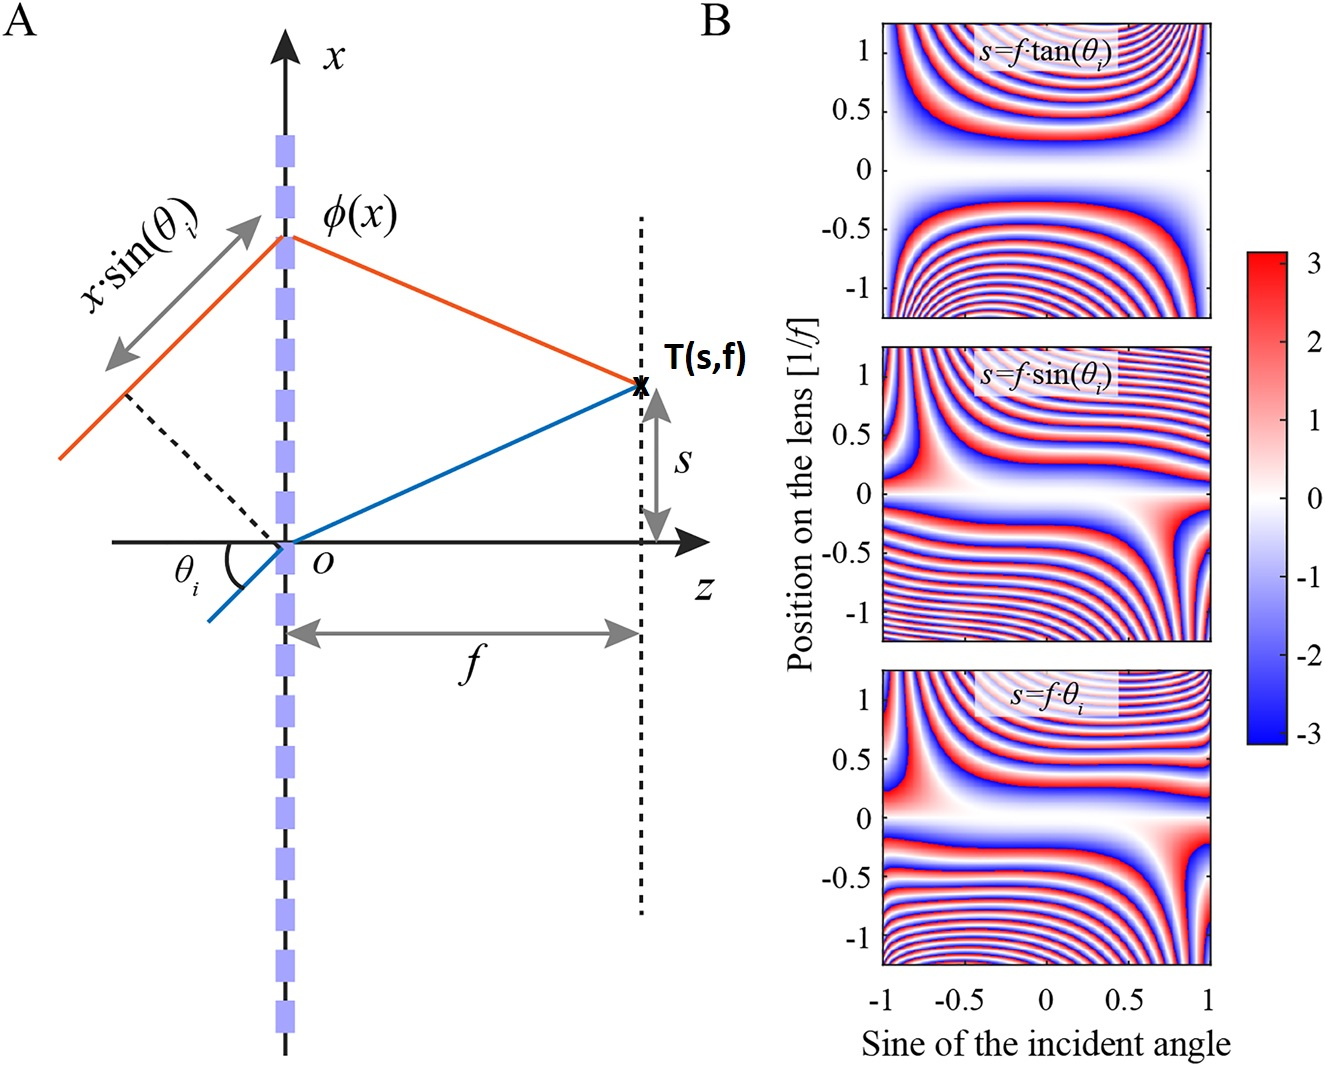
\includegraphics[width=9cm, height=7cm]{Slike/Gorisce.jpg}
     \caption{Slika A prikazuje lom svetlobe dveh različnih žarkov. Modri žarek pada v središče metaleče pod kotom $\theta_i$,  oranžni žarek pa opravi dodatno pot $x\sin(\theta_i)$. Zbereta se v točki T$(s, f)$. Slika B prikazuje fazne profile, ki morajo biti realizirani na metaleči, v odvisnosti od sinusa vpadnega kota. Podane so tri različne funkcije premika fokusa $s$ v odvisnosti od vpadnega kota $\theta_i$.  Vir: \cite{Goriscna} }
     \label{Hiperbolicna}
 \end{figure}
Na sliki \ref{Hiperbolicna}(B) lahko opazimo nekaj primerov faznega profila v odvisnosti od $\sin(\theta)$ in oddaljenosti od središča goriščne ravnine ($s/f$).  Zgornja slika nam prikazuje primer, ko se žarek sploh ne bi lomil. Torej bi bil vpadni kot enak lomnemu kotu in tako bi s slike \ref{Hiperbolicna}(A) lahko razbrali, da je $s=f\tan{\theta_I}$. Če bi to prikazovali na $x$ osi zgolj kot $\theta_i$, bi dobili vzporedne ravne črte faznega profila od $[-\pi,\pi]$, ampak teh ne dobimo zaradi prikaza $\sin(\theta_i)$. Srednja slika vzame primer $s=f\sin(\theta)$, ki ga uporabljajo Fourierove leče.\cite{primeri} \footnote{To so leče kjer se žarek po prehodu skozi lečo odziva kot na Fourierovo transformacijo.} Opazimo lahko, da je fazni profil za večje kote popačen, kar nam pove, da se širokokotnih metaleč hiperboličnega faznega profila ne more uporabljati za Fourierevo transformacijo svetlobe. Kot zadnji primer fazne ravnine je podan primer F-Theta leč s $s=f\theta$. Takšne leče se uporablja v rezalnih sistemih ali optičnih bralnikih. Te naprave so namreč izdelane tako, da delujejo pri majhnih kotih $\theta_i$, zato jim močna popačenost pri velikih vrednostih vpadnega kota ni pomembna. Ključno jim je zgolj to, da se v središču goriščne ravnine zbere največja intenziteta svetlobe \cite{F-theta}.\\
 
Drugi primer postavitve metalečnih struktur je metaleča, ki ustvarja kvadratični fazni profil. Enačbo faznega profila takšne leče smo izpeljali že v uklonu na krogelnih režah \eqref{Razlika}, kjer smo upoštevali, da so si izvor, leča in zaslon neskončno daleč in je bil tako kot $\theta_i$ majhen. V primeru, ko kot $\theta_i$ ni majhen, dobimo:
 \begin{equation}
    \phi\left(r, \theta_{\mathrm{i}}\right)=-\frac{k_{0}}{2 f} r^{2}-k_{0} x \sin \theta_{\mathrm{i}}=-\frac{k_{0}}{2 f}\left[\left(x+f \sin \theta_{\mathrm{i}}\right)^{2}+y^{2}\right]+\frac{k_{0} f \sin ^{2} \theta_{\mathrm{i}}}{2}.
\label{Kvadratična}
\end{equation}
Če si pogledamo desni del enačbe, vidimo, da imamo tako pri koordinati $x$ dodan še dodaten člen $f\sin(\theta_)$, ki povzroči, da se vsak vpadni žarek pod kotom $\theta_i$ zbere izven gorišča v točki $-f\sin(\theta_i)$. Tako se gorišče v premakne v odvisnosti od vpadnega kota.


  \begin{figure}[H]
     \centering
     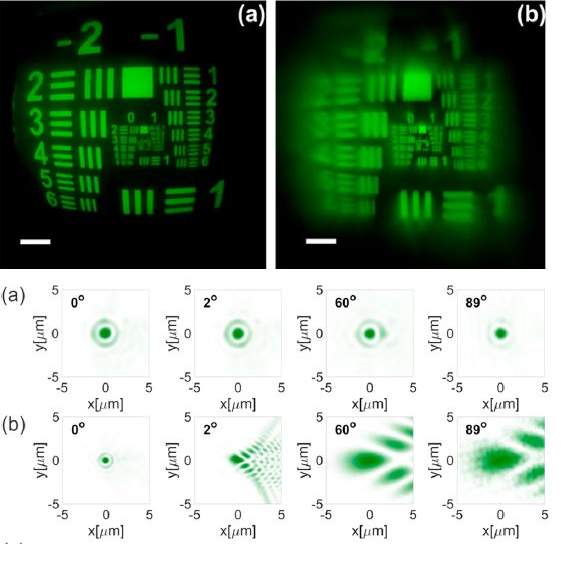
\includegraphics[width=8cm, height=7.5cm]{Slike/Fokusiranje.png}
     \caption{Zgornja slika prikazuje primerjavo med slikano številčnico s kvadratično širokokotno lečo (levo) in hiperbolično širokokotno lečo (desno). Spodnja slika prikazuje \textit{Point spread function} ali odziv leče na točkast izvor za posamično lečo (kvadratična zgoraj, hiperbolična spodaj), ko svetloba vpada pod različnimi koti.  Vir: \cite{Fokusiranje} }
     \label{Fokusiranje}
 \end{figure}

Zato se kvadratične leče uporablja za širokokotno slikanje. Za primer si lahko pogledamo sliko \ref{Fokusiranje} kjer je narejena primerjava med slikama, ustvarjenima s kvadratično in hiperbolično lečo ( \ref{Fokusiranje} zgoraj). Opazno je, da je pri širokokotni kvadratični leči slika jasna, pride pa do močnega popačenja, ki ga imenujemo \textit{fish-eye}. Ta se pojavi zaradi razlike v premiku zbiranja žarkov izven gorišča $-f\sin(\theta)$. Ker pa vemo, kolikšna bo vrednost odmika zbiranja žarkov v vsaki točki, lahko to napako računalniško odpravimo. Medtem pri hiperbolični leči lahko opazimo, da pride do zamegljenosti že pri nizkih kotih, medtem ko v središču dobimo boljšo ločljivost. Razlog za zamegljenost izhaja iz tega, da pride pri pri velikih kotih pri hiperbolčni leči do velikega popačenja v faznem profilu (glej desno sliko \ref{Hiperbolicna}). Tako vidimo, da takšna leča ni primerna za slikanje širokokotnih slik. Njena prednost pred kvadratičnim faznim profilom pa se dobro pokaže pri sliki \ref{Fokusiranje} spodaj, kjer je intenziteta svetlobe hiperbolične leče pri ničelnem kotu večja kot pri kvadratični leči, vendar že pri nizkih kotih ne dobimo dobrega zbiranja zgolj v eni goriščni ravnini \cite{Fokusiranje}.

 



\subsubsection{Faza in interferenca}
Optične površine svetlobo prepuščajo, lomijo in odbijajo glede na njihov lomni količnik in sprememba faze pa se ustvarja skozi celotno pot v snovi. Pri metaleči pa fazo vpadne svetlobe spremenimo takoj na površini s pomočjo faznega-gradienta. Ta povzroči, da vpadna svetloba, na različnih vpadnih pravokotnicah prejme različni fazni zamik. To obnašanje opiše posplošeni lomni (Snellov) zakon. 
 \\
 
 \begin{figure}[H]
     \centering
     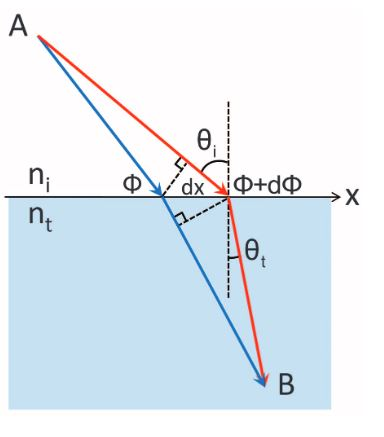
\includegraphics[width=7cm, height=8cm]{Slike/Sneel.JPG}
     \caption{ Prikaz loma svetlobe na površini z različnima lomnima količnikoma z upoštevanjem dodatka fazne razlike. Vir: \cite{Snell} }
     \label{Snell}
 \end{figure}
 
 Vzemimo dva žarka iz istega izvora, močno oddaljenega od leče, ki sta pri vpadu na mejno površino med seboj oddaljena za razdaljo $\text{d}x$, kot prikazuje slika \ref{Snell}. Ko se bosta dana žarka po prehodu v snov srečala v točki B, bosta ustvarila konstruktivno interferenco takrat, ko je razlika njunih faz enaka 0:
 \begin{equation}
     \left[k_0n_i\sin(\theta_i)\text{d}x+(\Phi+\text{d}\Phi)\right]-\left[k_0n_t\sin(\theta_t)\text{d}x+\Phi\right]=0,
 \end{equation}
 kjer je $\theta_t$ lomni kot, $\Phi$ in $\text{d}\Phi$ pa dodatna fazna zamika  posameznih valov, zaradi prehoda v snov pri različni vpadni pravokotnici. Če enačbo preuredimo, dobimo 
 \begin{equation}
     \left[k_0n_i\sin(\theta_i)-k_0n_t\sin(\theta_t)\right]\text{d}x=-\left(\text{d}\Phi\right).
 \end{equation}
 Če sedaj enačbo delimo z $\text{d}x$, lahko prepoznamo definicijo odvoda. Sledi
 \begin{equation}
\sin \left(\theta_{\mathrm{t}}\right) n_{\mathrm{t}}-\sin \left(\theta_{\mathrm{i}}\right) n_{\mathrm{i}}=\frac{\lambda_{\mathrm{o}}}{2 \pi} \frac{d \Phi}{d x},
\label{Snelov}
\end{equation}
čemur pravimo tudi generalizirani Snellov zakon za lom svetlobe \cite{Snell}. S podobnimi razmisleki bi lahko izpeljali tudi odbojni zakon
 \begin{equation}
\sin \left(\theta_{\mathrm{r}}\right) -\sin \left(\theta_{\mathrm{i}}\right) =\frac{\lambda_{\mathrm{o}}}{2 \pi n_i} \frac{d \Phi}{d x},
\end{equation}
kjer je $\theta_r$ kot odboja.

Pri enačbi \eqref{Snelov} opazimo, da zveza med $\sin(\theta_r)$ in $\sin(\theta_i)$ ni več le razmerje med lomnimi količniki, ampak se je pojavil dodaten člen spreminjanja faze v odvisnosti od kraja. V primeru, ko je dodatna faza neodvisna od kraja na leči, $d \Phi/d x=0$, bi dobili navadni Snellov zakon \cite{Snell}.\\


Tako lahko ustvarjamo interference odbitih in vpadnih valov na več možnih načinov, na primer z uporabo elektromagnetnih praznin, nanodelčnih struktur ali plazmonskih anten. Za popoln nadzor nad valovno fronto mora biti snov sposobna ustvarjati fazni zamik od 0 pa vse do $2\pi$.

 
 
 \begin{figure}[H]
     \centering
     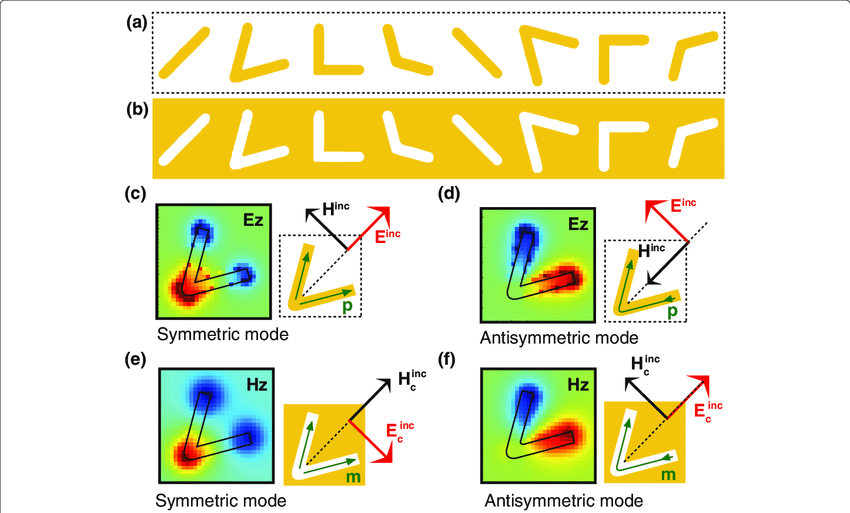
\includegraphics[width=11cm, height=6.7cm]{Slike/Antenna.png}
     \caption{Slika prikazuje postavitve in primere plazmonskih nanoanten. (a) in (b) predstavljata postavitev V-anten in V-vrzeli v sredstvu, da ustvarijo fazni zamik za $2\pi$, (c) in (e) predstavlja primer simetrične antene in vrzeli, medtem ko (d) in (f) predstavlja antisimetrično anteno in vrzel. Zelene puščice nam prikazujejo inducirani dipolni moment, barvno ozadje pa prikazuje jakost polja, ki ga ta ustvarja. Z črno in rdečo puščico sta narisana magnetno in električno polje vpadnega valovanja. Vir: \cite{Antena}. }
     \label{Antena}
 \end{figure}
 
Za prvo eksperimentalno realizacijo generaliziranega Snellovega zakona so bile uporabljene vrstice plazmonskih nanoanten v obliki črke V v srednjem in bližnjem infrardečem območju (slika \ref{Antena}). Antene so sestavljene iz dveh krakov iste dolžine, ki sta združena, da tvorita kot $\Delta$. V primeru ko na njih svetimo s svetlobo z amplitudo elektro-magnetnega polja $E_{inc}$ in $H_{inc}$, pride v anteni do resonančnega odziva.  Antene imajo tako dva lastna nihajna načina; simetrični (slika \ref{Antena} (c),(d)) ali antisimetrični (slika \ref{Antena} (e),(f)). Te dva sta določena glede na smer induciranega dipolnega momenta. Če definiramo vektor orientacije antene, nam bo ta za simetričen način razpolavljal kot med krakoma, medtem ko bo v antisimetričnem načinu kazal med krakoma. Da vemo, ali antena ustvari resonančni odziv zaradi magnetnega ali električnega polja, si moramo pogledati, katero polje je vzporedno z vektorjem orientacije. Tako lahko razberemo, da imajo antene, \ref{Antena}(c) in (d), električen nihajni način in vrzeli, \ref{Antena}(e) in (f), magnetni nihajni način.  \cite{Antena}, \cite{Snell}.


\begin{figure}[H]
\centering
  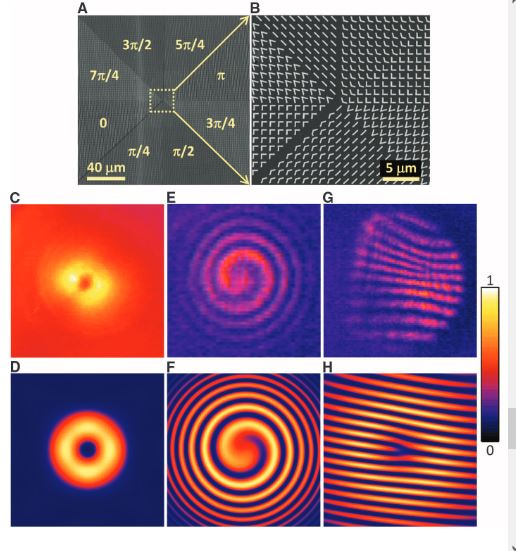
\includegraphics[width=.7\linewidth, height=9cm]{Slike/Faza.JPG}
  \caption{Slika prikazuje (A) spremembo faze anten in (B) približan prikaz zgradbe metapovršine. (C) in (D) nam prikazujeta izmerjeno in izračunano intenziteto svetlobe vorteksa z indeksom $m=1$, ki jo ustvari dana leča, če nanjo svetimo z linearno polarizirano svetlobo. (E) in (F) prikazujeta primer, ko na lečo svetimo z kombinacijo linearno polarizirane svetlobe in Gaussovega žarka in rezultat lečenja je spirala. (G) in (H) pa prikazujeta primer, ko v kombinaciji linearno polarizirane svetlobe in Gaussovega žarka, enega izmed njiju zamaknemo od središča za manjši kot in tako lahko opazimo oba pojava hkrati (pojav obroča in ločenja črt).   Vir: \cite{Snell}  }
  \label{Faza}
\end{figure}

Fazo valovanja s takimi strukturami nadziramo tako, da  spreminjamo orientacijo in obliko nanoanten, predvsem kot med krakoma. Pri spreminjanju kota pa moramo biti predvsem pazljivi na to, da ta ni prevelik (saj bo tako električno-magnetni dipol, ki ga ustvarja antena, prešibek) in ne premajhen (ker bi tako prišlo do sklopitve polj med antenami, \textit{field-coupling}, kar bi vplivalo na spremembo faze in amplitude posamezne antene). V primeru V-anten bi potrebovali osem zaporednih valovnih anten z različnimi koti in orientacijami, kot prikazuje slika \ref{Antena}(a), da bi lahko svetlobi spremenili fazni zamik za $2\pi$ \cite{Antena}. Primer ustvarjanja faznega zamika linearno polariziranemu vpadnemu valovanju lahko opazimo na sliki \ref{Faza}. 





 
\subsection{Preprosta izdelava metaleč}
Zaenkrat smo govorili zgolj o osnovnih načelih, ki jim mora metaleča zadoščati, da zbira svetlobo in da uspe ustvarjati fazni zamik, nič pa še nismo govorili o sami izdelavi metaleč in problemih, s katerimi se soočamo v praksi.

Iz enačbe \eqref{Razlika} razberemo, da je goriščna razdalja leče odvisna od tega, kolikšna je valovna dolžina vpadne svetlobe. Zato se je v raziskovanju metaleč veliko pozornosti posvečalo izdelavi leč, ki bi svetlobe različnih valovnih dolžin zbirale v isti goriščni ravnini. 

 \begin{figure}[H]
     \centering
     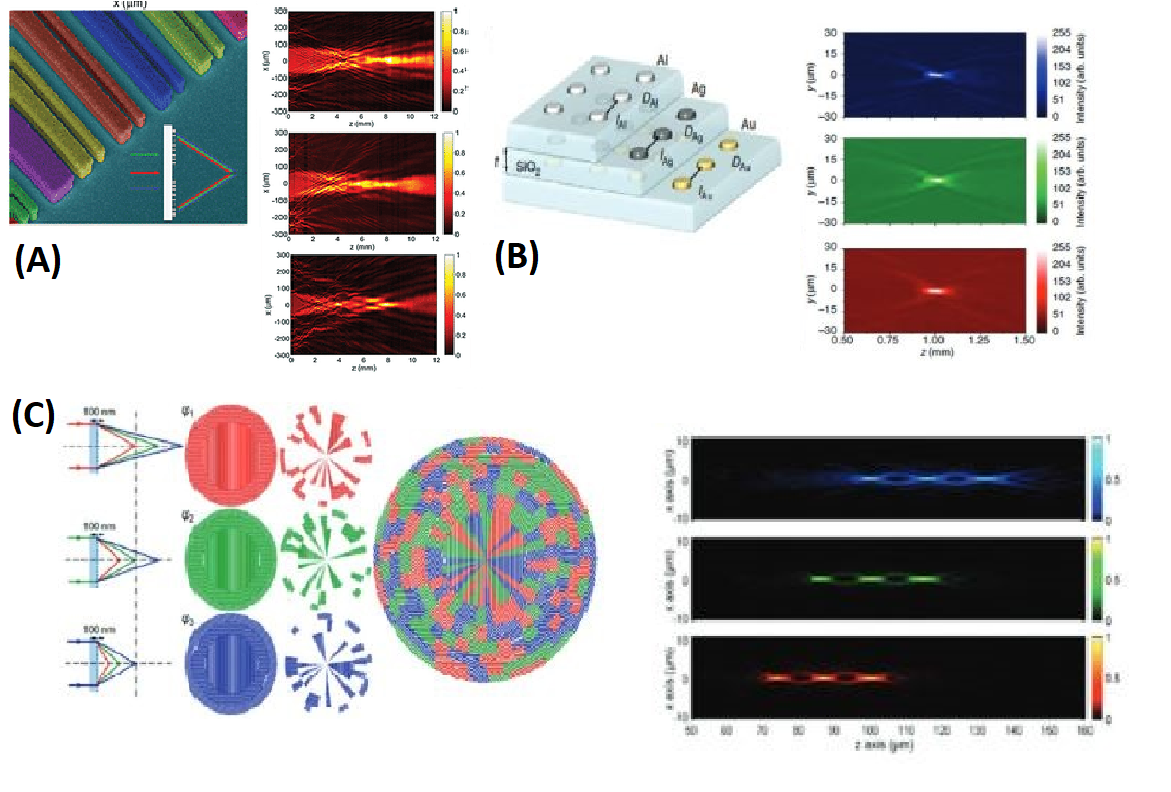
\includegraphics[width=13cm, height=10cm]{Slike/Lece.png}
     \caption{Slika prikazuje primere sestavljenih metapovršin. (A) predstavlja metalečo, zgrajeno iz podolgovatih dielektričnih resonatorjev (levo), ki lomijo svetlobo valovne dolžine 1300 nm (zgoraj desno), 1550 nm (v srednini desno) in 1800 nm (spodaj desno). Slika (B) prikazuje triplastno lečo iz zlata, aluminija in srebra (zgoraj levo), ki je sposobna lomiti svetlobe valovnih dolžin 650 nm, 550 nm in 450 nm (desno). Slika (C) prikazuje sestavljeno lečo iz treh različnih posameznih metaleč. Posamezne metaleče so prikazane na sliki levo , sestavljena leča pa je prikazana desno. Najbolj desno lahko vidimo, kako takšna leča zbira svetlobo posamezne valovne dolžine rdeče, modre in zelene svetlobe.  Vir: \cite{Metaleče_opis}  }
     \label{Geometrija}
 \end{figure}
 
 Prvi primeri reševanja tega problema so bili bolj preproste narave, in sicer kot skupek metaleč, kjer posamezna metaleča lomi svetlobo specifične valovne dolžine v skupnem gorišču. Enega izmed takšni primerov lahko vidimo na sliki \ref{Geometrija} (A).  Cappasso in njegovi sodelavci \cite{Metaleče_opis} so s pomočjo horizontalnega zlaganja pravokotnih dielektričnih resonatorjev sestavili metalečo, ki je sposobna usmeriti svetlobo v isto goriščno ravnino za tri različne valovne dolžine; $\lambda= 1300, 1550, $ in $1800$ nm. Druga možnost postavitve je bila vertikalno zlaganje metaoptičnih površin. Kot primer je na sliki \ref{Geometrija}(B) prikazana metaleča, sestavljena treh vertikalno zloženih plasti, ki zbirajo svetlobo valove dolžine 650 nm, 550 nm in 450 nm. Vsaka plast je sestavljena iz gradnikov v obliki nanodiska, ki so zgrajeni iz različni materialov (aluminija, zlata in srebra). Tretji način postavitve pa lahko opazimo na sliki \ref{Geometrija} (C), kjer metaleča zbira svetlobo valovnih dolžin (480, 550 in 620 nm). V tem primeru so bile najprej izdelane tri različne metaleče, vsaka za svojo valovno dolžino in nato razdeljene v segmente, ki so jih naključno razporedili po metapovršini. Z naključno postavitvijo so tako lahko dosegli boljše zbiranje svetlobe v goriščni razdalji \cite{Metaleče_opis}.\\
 
 Zaradi napredka v cenejšem in bolj natančnem izdelovanju metapovršin se je močneje začelo razvijati tudi akromatično\footnote{Akromatične leče so leče, ki zbirajo svetlobo pasu valovnih dolžin v goriščni ravnini.} zbiranje svetlobe. Enega izmed takšnih primerov akromatične metaleče si lahko pogledamo na sliki \ref{Geometrija-Lec}(A), kjer je leča narejena iz nanostolpcev titanovega dioksida (TiO$_2$) in kovinskih ogledalc, ki jih loči med seboj pas dielektrika. Takšna leča je sposobna pri konstantni valovni dolžini zbrati svetlobo od $\lambda$=490 do 550 nm. Iz izračunov so uspeli ugotoviti tudi, da lahko z različnimi debelinami stolpcev ustvarijo različne fazne zamike za posamezne valovne dolžine in privedejo do boljše interference.
 
   \begin{figure}[H]
     \centering
     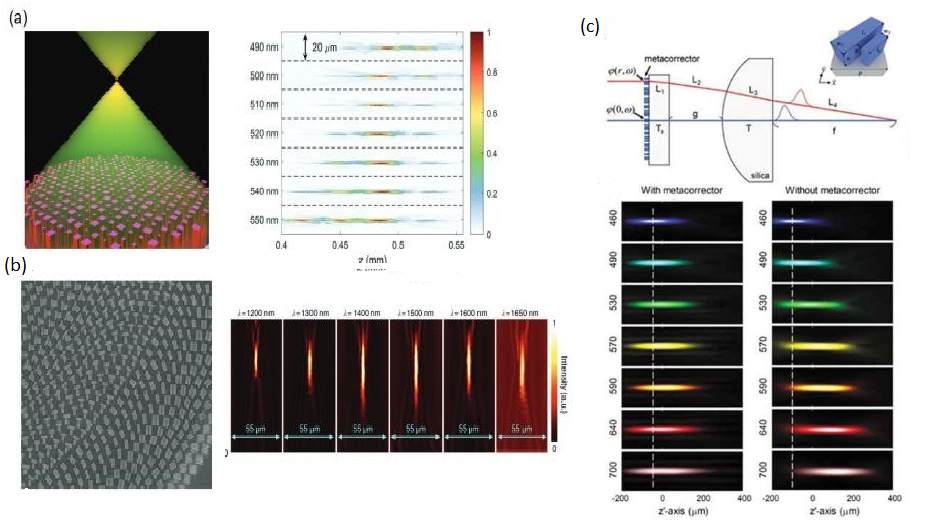
\includegraphics[width=12cm, height=8cm]{Slike/Spektrometri.png}
     \caption{Slika prikazuje primere metapovršin, ki s pomočjo nanostruktur zbirajo svetlobo. (A) predstavlja metalečo, zgrajeno iz stolpcev titanovega dioksida (leva slika), ki pri konstantni goriščni razdalji 0.4 mm (desna slika) zbira svetlobo od 490 nm pa do 550 nm. (B) predstavlja primer leče zgrajene iz IRU struktur (leva slika), ki lomijo svetlobo valovnih dolžin 400-667 nm v isti goriščni razdalji (desna slika). (C) nam prikazuje sestav metaleče z dodatkom metakorektorja iz titanovega dioksida (zgoraj) in nato grafičen prikaz zbiranja svetlobe brez korektorja (spodaj levo) in s korektorjem (spodaj desno). Vir: (A) in (B) \cite{Metaleče_opis}, (C) \cite{Geometrija-dodatek} }
     \label{Geometrija-Lec}
 \end{figure}
 Pred kratim pa so Tsai in sodelavci oblikovali metalečo iz resonančnih struktur, ki se imenujejo IRU. Strukture so zgrajene s posebej urejenimi delci zlatih nanopaličic, SiO$_2$ ploščic in Au refraktorskih ploščic (glej sliko \ref{Geometrija-Lec}(B)). Z pravilnim oblikovanjem metapovršine iz resonančnih nanostruktur lahko dosežemo različne fazne razlike. Podobno strukturo so nato zgradili tudi iz Aluminijastih refraktorskih ploščic, saj ima ta višjo plazemsko frekvenco in je zato njegova absorpcija v vidni svetlobi manjša, kar vodi k boljšemu izkoristku za valovne dolžine od 400 do 667 nm.

 
 Da bi lahko popravili spreminjanje goriščne razdalje zaradi spreminjanja valovne dolžine svetlobe, se ponavadi uporabljajo kromatični fazni kompenzatorji ali metakompenzatorji. Tako lahko s pravilno obliko metakorektorja iz titanovega dioksida, ki ga postavimo za lečo, precej izboljšamo zbiranje svetlobe v goriščni razdalji, hkrati pa tudi povečamo območje zbiranja valovnih dolžin. Če uporabimo ta dodatek pri naši leči, zgrajeni iz Ai, lahko iz slike \ref{Geometrija-Lec}(C) opazimo, da je goriščna razdalja takšne metaleče za vso vidno svetlobo skoraj enaka \cite{Geometrija-dodatek}.
 

 
 \section{Uporaba metaleč v praksi}
 Kot optične naprave imajo metaleče zaradi svoje tankosti in kompaktnosti veliko prednosti v primerjavi s standardnimi lečami in lahko z njimi rešimo veliko optičnih problemov, ki jih s klasičnimi lečami ne moremo. V tem poglavju bomo preučili uporabo metaleč v določenih področjih optike (slikanje, spektroskopija, barvno usmerjanje ...) in zraven razmislili o izboljšavah metaleč. 
 \subsection{Slikanje}
 Vemo, da človek največ informacij iz zunanjega sveta prejme ravno prek vida; optičnega sistema leč, ki se je z milijoni let evolucije izpopolnil za fokusiranje in projeciranje barvnih slik na mrežnico. Metaleče se zaenkrat tako dobremu lečenju kot oko še niso približale, problemi pa se pojavijo predvsem v kvaliteti slike, saj je izkoristek sistema zaradi absorpcije svetlobe v leči dokaj slab. Kljub temu so znanstveniki že uspeli doseči 80 \% izkoristek metaleče, vendar na račun povečanja kompleksnosti optičnega sistema leč in refraktorjev. Za gradnjo takšnih sistemov se ponavadi uporablja predvsem titanov oksid (TiO$_2$) in galijev nitrit (GaN), ki sta zaradi svoje visoke vrednosti dielektrične konstante sposobna dosegati visoke vrednosti izkoristkov tudi do 86 \%.
 
 Na žalost pri metalečah še vedno lahko vidimo močno kromatično aberacijo, kar pomeni, da je opazna razlika med slikami posnetimi s svetlobo različnih valovnih dolžin. Opazi se, da je fazni profil za različne valovne dolžine drugačen in zato je slika barvno razmazana, popačena. Nekaj primerov si lahko ogledamo na sliki \ref{Ptica}. Slika \ref{Ptica} (a) prikazuje majhno številčnico, kjer je posamezna paličica velikosti približno 40 $\mu$m. Slikali so jo z dvema različnima metalečama; Ga-N in TiO$_2$ metalečo. Najprej so prikazane slike narejene s TiO$_2$ metalečo (\ref{Ptica} (b)), kjer je številčnica sevala različne valovne dolžine (480 nm, 530 nm, 590 nm in 620 nm), nato pa je prikazan kompozitum vseh štirih slik za Ga-N lečo \ref{Ptica} (c). Za vsako valovno dolžino je številčnica, kljub svoji majhnosti, dobro vidna, vendar se pri uporabi Ga-N metaleče za primer slikanja večjih objektov, kot je na primer ptica na sliki \ref{Ptica} (d), barve popačijo prav zaradi kromatične aberacije. Zato je zaenkrat slikanje s pomočjo metaleč še zelo odprto področje za raziskovanje in napredek \cite{Metaleče_opis}.
 
  \begin{figure}[H]
     \centering
     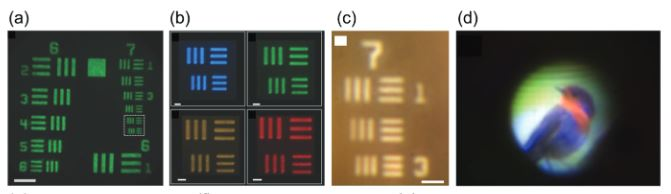
\includegraphics[width=14cm, height=5cm]{Slike/Ptica.JPG}
     \caption{Primeri slikanja z metalečami. (a) Primer številčnice, ki sveti s 530 nm, ki so jo slikali z metalečo, narejeno iz TiO$_2$. (b) Isti primer, le da so tokrat uporabili svetlobe drugih valovnih dolžin (480 nm, 530 nm, 590 nm in 620 nm). (c) Sestavljena slika valovnih dolžin treh različnih svetlob, slikanih z metalečo, zgrajeno iz Ga-N molekul. Kljub majhnosti slike so podrobnosti še vedno razvidne, vendar je slika vseeno rahlo popačena. Popačenost se poveča pri slikanju večjih objektov, kar prikazuje slika (d), kjer je z Ga-N metalečo slikana ptica Erithacus rubecula. Vir: \cite{Metaleče_opis}. }
     \label{Ptica}
 \end{figure}
 
 \subsection{Spektroskopija}
 Medtem ko večini optični sistemov disperzija svetlobe, ki jo ustvarja metaleča, prinaša negativen učinek, pa se v določenih optičnih napravah disperzijo uporablja za izboljšanje delovanja naprave. Kot primer lahko vzamemo spektroskope, kjer je za izboljšanje njihove ločljivosti potrebna velika optična pot svetlobe od leče od detektorja. Razlog za to je v tem, da se z daljšanjem optične poti v snovi, povečuje razlika v legi točke zbiranja svetlobe za različne valovne dolžine (slika \ref{Spekter}(a)). Tako lahko lažje razločimo intenzitete posameznih valovni dolžin, vendar pa povečujemo velikost samega spektroskopa. Zato so začeli v spektroskopiji uvajati sisteme, sestavljene iz metaleč, ki so sposobne razločevati svetlobo različnih valovnih dolžin z visoko resolucijo. Tako se za lečo doda dodatno metalečo, slika \ref{Spekter}, zgrajeno iz silikonskih nanostruktur TiO$_2$, ki ustvarijo fazni zamik in povzročijo zbiranje svetlobe posamezne valovne dolžine v določeni točki \cite{Metaleče_opis}.
 
  \subsection{RGB filtri in senzorji}
 Zaradi svoje majhnosti in praktičnosti ločevanja barv pri različnih valovih dolžinah se je uporabnost metaleč ponudila tudi v CMOS\footnote{\textit{Complementary Metal Oxide Semiconductor}.} senzorjih (slika  \ref{Spekter}(c)). Že večkrat omenjena Ga-N dielektrična metaleča bi lahko znotraj filtra delovala kot usmerjevalnik treh glavnih barv; rdeče (420 nm) modre (532 nm) in zelene (633 nm) svetlobe in vsako fokusirala pri svoji goriščni razdalji. Ker takšna metaleča pri teh valovnih dolžinah deluje z izkoristkom do 87 \%, bi dodatek metaleče znotraj optičnega sistema CMOS detektorjev močno izboljšal resolucijo obdelave barv v sliki \cite{Metaleče_opis}.
 
  \begin{figure}[H]
     \centering
     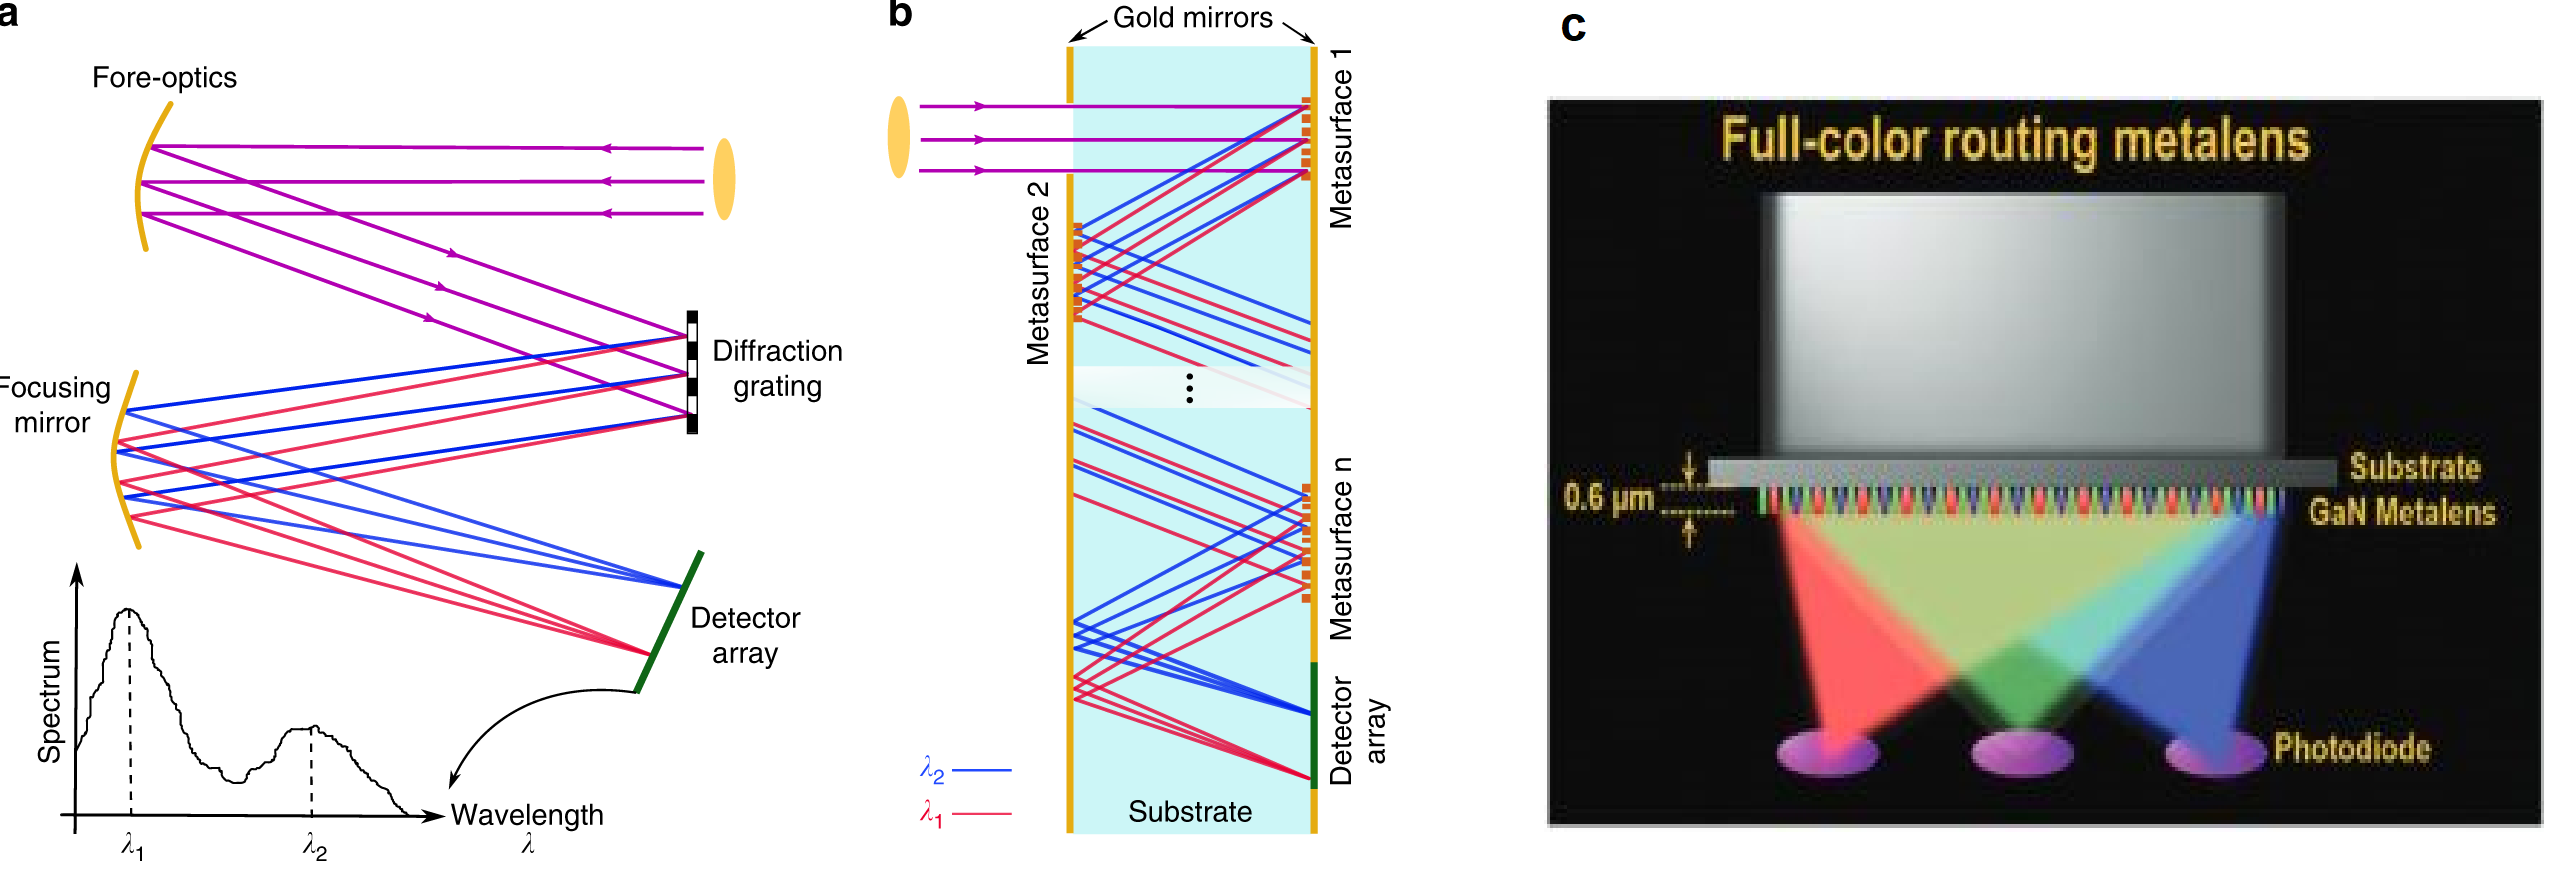
\includegraphics[width=15cm, height=7cm]{Slike/Spektrometer 2.png}
     \caption{Slika prikazuje primera izvedbe spektrometra: (a) prikazuje spektrometer, kjer se svetlobo ukloni na uklonski mrežici in nato zbere s pomočjo dodatnega zrcala, (b) prikazuje spektrometer, izdelan iz metaleč, ki odbija ter lomi svetlobe znotraj sistema metapovršin in (c) prikazuje implementacijo metaleče v sistem s CMOS detektorjem. Vir: (a) in (b) \cite{Spektroskop}, (c) \cite{Metaleče_opis}. }
     \label{Spekter}
 \end{figure}
 


\section{Zaključek}
Metaleče so ultratanke optične površine, ki zagotavljajo kontrolo različnih lastnosti svetlobe, kot so faza, polarizacija in amplituda. S tem predstavljajo alternativo klasičnim optičnim lečam, ki so zaradi svoje velikosti v optičnih napravah postale precej okorne in se jim z drugimi alternativami želimo izogniti. Optične lastnosti metaleč izvirajo iz postavitve nanostruktur znotraj le-teh. Kot smo spoznali, je ključna razporeditev nanostruktur znotraj leče, da te zagotavljajo konstruktivno interferenco pri goriščni razdalji. Za postavitev struktur se ponavadi uporabljata hiperbolični ali kvadratični profil faznega zamika, ki zagotovita zbiranje svetlobe v goriščni razdalji $f$. Sama oblika struktur in njihova postavitev je pomembna za spreminjanje faze valovanja, ki gre skozi metalečo. Tako smo spoznali, da lahko z različno postavitvijo istih struktur znotraj metaleče ustvarimo drugače polarizirano svetlobo ali pa optični vorteks. 


Za samo izdelavo metaleče je pomembno vedeti, za kaj jo bomo potrebovali. Ker je fazni zamik metaleče odvisen od valovne dolžine, se tako svetloba različnih barv zbira v različnih goriščnih ravninah. Raziskovalci so se poskušali temu izogniti na več načinov, in sicer z gradnjo struktur iz večih metaleč, pri čemur vsaka lomi svetlobo določene valovne dolžine v goriščni ravnini $f$, ali pa z dodajanjem dodatnih metakorektorjev, ki pomagajo pri razširitvi spektra delovanja leče. Prav zaradi te lastnosti zaenkrat še niso prišle v uporabo za slikanje različnih objektov, saj se pri večjih objektih resolucija leče močno pokvari in se barve med seboj razmažejo. 

Kljub temu ima ta efekt tudi prednosti, ki jih izkoriščajo v spektroskopiji. Zaradi dobre sposobnosti razločevanja svetlobe pri posamezih valovnih doližinah se je tako metaleče začelo uporabljati za izboljšanje filtriranja svetlobnega spektra in tako močno izboljšalo resolucijo spektroskopov.  

Čeprav je zaenkrat malo verjetno, da bodo metaleče v celoti nadomestile klasične optične elemente, pa predstavljajo dober korak v fazi razvoja tankih optičnih površin in integracijo teh v optične naprave.


\printbibliography





\end{document} 